\documentclass[12pt]{article}
\usepackage{{../preamble}}
\graphicspath{{pics}}

\begin{document}
\chead{Problem Set 3}

%%%%%%%%%%%%%%%%%%%%%%%%%%%%%%%%%%%%%%%%%%%%%%%
%                  Definitions                %
%%%%%%%%%%%%%%%%%%%%%%%%%%%%%%%%%%%%%%%%%%%%%%%
\def\xdot{\dot X} \def\ydot{\dot Y} \def\zdot{\dot Z}
\def\kdot{\dot k} \def\ccdot{\dot c} \def\ddt{\frac{d}{dt}}
\def\dfdk{\frac{\partial F}{\partial K}}
\def\dfdl{\frac{\partial F}{\partial L}}
\def\plim{\lim\limits_{\phi\to 0}}
\def\ddp{\dfrac{\partial}{\partial \phi}}
\def\dgdp{\dfrac{\partial\gamma}{\partial \phi}}
\def\invphi{\sfrac{1}{\phi}}
\def\kone{k^*_1} \def\ktwo{k^*_2}




%%%%%%%%%%%%%%%%%%%%%%%%%%%%%%%%%%%%%%%%%%%%%%%
%                Problem 1                    %
%%%%%%%%%%%%%%%%%%%%%%%%%%%%%%%%%%%%%%%%%%%%%%%
\section*{Problem 1}
\problem{The elasticity of substitution with constant-relative-risk-aversion utility: Romer 2.2}{
    Consider an individual who lives for two periods and whose utility is given by equation (2.43). Let $P_1$ and $P_2$ denote the prices of consumption in the two periods, and let $W$ denote the value of the individual’s lifetime income; thus the budget constraint is $P_1C_1 + P_2C_2 = W$.

    \begin{enumerate}[label=(\alph*)]
    \item What are the individual’s utility-maximizing choices of $C_1$ and $C_2$, given $P_1$, $P_2$, and $W$?
    \end{enumerate} 
}




%%%%%%%%%%%%%%%%%
%     Part b    %
%%%%%%%%%%%%%%%%%
\newpage\problem{}{
    \begin{enumerate}[label=(\alph*)]
    \setcounter{enumi}{1}
    \item The elasticity of substitution between consumption in the two periods is
$-[(P_1/P_2)/(C_1/C_2)][\partial(C_1/C_2)/\partial(P_1/P_2)]$, or $-\partial \ln (C_1/C_2)/\partial \ln (P_1/P_2)$. Show that
with the utility function (2.43), the elasticity of substitution between $C_1$ and
$C_2$ is $1/\theta$.
    \end{enumerate} 
}







%%%%%%%%%%%%%%%%%%%%%%%%%%%%%%%%%%%%%%%%%%%%%%%
%                Problem 2                    %
%%%%%%%%%%%%%%%%%%%%%%%%%%%%%%%%%%%%%%%%%%%%%%%
\newpage
\section*{Problem 2}
\problem{Find the utility-maximizing path of $C$: Romer 2.5}{
    Consider a household with utility given by (2.2) (2.3). Assume that the real interest
rate is constant, and let $W$ denote the household’s initial wealth plus the present
value of its lifetime labor income (the right-hand side of [2.7]). Find the utility-maximizing path of $C$, given $r$, $W$, and the parameters of the utility function.
}












%%%%%%%%%%%%%%%%%%%%%%%%%%%%%%%%%%%%%%%%%%%%%%%
%                Problem 3                    %
%%%%%%%%%%%%%%%%%%%%%%%%%%%%%%%%%%%%%%%%%%%%%%%
\newpage
\section*{Problem 3}
\problem{Using the phase diagram to analyze the impact of an anticipated change: Romer 2.11}{
    Consider the policy described in Problem 2.10, but suppose that instead of announcing and implementing the tax at time 0, the government announces at time 0 that at some later time, time $t_1$, investment income will begin to be taxed at rate $\tau$.

    \begin{enumerate}[label=(\alph*)]
        \item Draw the phase diagram showing the dynamics of $c$ and $k$ after time $t_1$.
    \end{enumerate} 
}
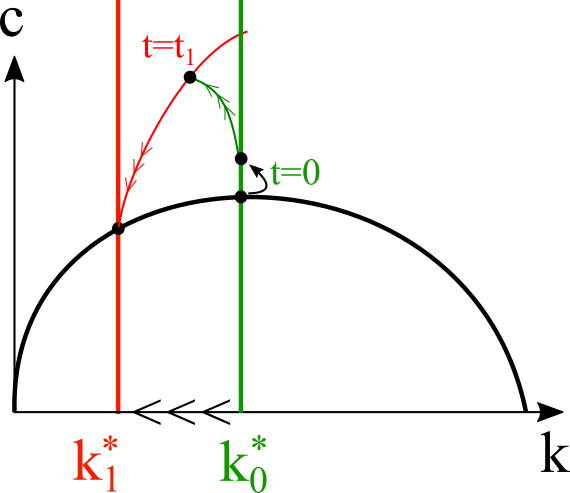
\includegraphics[width=0.8\textwidth]{3.a}



%%%%%%%%%%%%%%%%%
%     Part b    %
%%%%%%%%%%%%%%%%%
\problem{}{
    \begin{enumerate}[label=(\alph*)]
    \setcounter{enumi}{1}
    \item Can $c$ change discontinuously at time $t_1$? Why or why not?
    \end{enumerate} 
}




%%%%%%%%%%%%%%%%%
%     Part c    %
 %%%%%%%%%%%%%%%%% \newpage
\newpage
\problem{}{
    \begin{enumerate}[label=(\alph*)]
    \setcounter{enumi}{2}
    \item Draw the phase diagram showing the dynamics of $c$ and $k$ before $t_1$.
    \end{enumerate} 
}





%%%%%%%%%%%%%%%%%
%     Part d    %
%%%%%%%%%%%%%%%%%
\newpage\problem{}{
    \begin{enumerate}[label=(\alph*)]
    \setcounter{enumi}{3}
    \item In light of your answers to parts (a), (b), and (c), what must $c$ do at time 0?
    \end{enumerate} 
}




%%%%%%%%%%%%%%%%%
%     Part e    %
%%%%%%%%%%%%%%%%%
\newpage\problem{}{
    \begin{enumerate}[label=(\alph*)]
    \setcounter{enumi}{4}
    \item Summarize your results by sketching the paths of $c$ and $k$ as functions of time.
    \end{enumerate} 
}






\end{document}

